\documentclass[letterpaper, 12pt]{article}

\usepackage[utf8]{inputenc}
\usepackage[english, spanish]{babel}
\usepackage{fullpage}
\usepackage{graphicx}
\usepackage{amsmath}
\usepackage{enumitem}
\usepackage{chngcntr}
\usepackage{setspace}
\usepackage{url}
\usepackage{csquotes}
\usepackage{float}
\usepackage{verbatim}
\usepackage{tabularx}
\usepackage{amsmath}
\usepackage{caption}
\usepackage{bm}
\usepackage{colortbl}
\usepackage{xcolor}
\usepackage{multicol}
\usepackage{wrapfig}
\usepackage{multirow}

% \usepackage{hyperref}

\counterwithin{figure}{section}
\renewcommand{\thesection}{\arabic{section}}
\renewcommand{\thesubsection}{\thesection.\arabic{subsection}}
\renewcommand{\baselinestretch}{2}

\usepackage[style=numeric, maxnames=6, minnames=3, backend=biber, parentracker=true, sorting=none]{biblatex}
\DefineBibliographyStrings{english}{%chktex-file 1 chktex-file 6
      andothers = {\em et\addabbrvspace al\adddot}
}
\addbibresource{./Bibliography/bibliography.bib}

\usepackage{array}

\setlength{\parskip}{0pt}

\raggedbottom{}

\newcommand{\bolditalic}[1]{\textbf{\textit{#1}}}

\begin{document}

\begin{titlepage}
      \centering
      
\includegraphics[width=0.3\textwidth]{Images/logo_utb.png}\par\vspace{1cm}
      {\scshape\LARGE Universidad Tecnológica de Bolívar \par}
      \vspace{.5cm}

      {\scshape\Large FÍSICA CALOR Y ONDAS \par}
      \vspace{.2cm}

      % chktex-file 8
      {\scshape\Large Grupo 1 \par}
      \vspace{.5cm}
      % chktex-file 8
      \slshape {\Large \bfseries{}Informe de Laboratorio No. VIII\\}
      \slshape {\small \bfseries{}EFECTO COMPTON \\ {Verificación de la perdida de energía de los fotones dispersados}}
      \vspace{1cm}

      \slshape {\itshape{} Mauro González, T00067622 \\}
      \slshape {\itshape{} German De Armas Castaño, T00068765 \\}
      \slshape {\itshape{} Angel Vega Rodriguez, T00068186 \\}
      \slshape {\itshape{} Juan Jose Osorio Ariza, T00067316 \\}
      \slshape {\itshape{} Jorge Alberto Rueda Salgado, T00068722 \\}
      \vfill
      Revisado Por \\
      Duban Andres Paternina Verona\\
      {\large \today\par}
\end{titlepage}

% chktex-file 44
% chktex-file 24

% ! ----------------------------------------------------------------------|>
\section{Introducción}

El efecto Compton, descubierto por el físico estadounidense
A.H. Compton en 1923~\cite{el_efecto_compton}, marcó un
hito fundamental en la comprensión de la naturaleza
corpuscular de los rayos X. Este fenómeno, que involucra la
dispersion de fotones por electrones, evidencia un cambio
en la longitud de onda de la radiación dispersada. La
practica experimental busca verificar cuantitativamente el
efecto Compton utilizando radiación gamma y analizar sus
implicaciones en términos de conservación de energía y
cantidad de movimiento

% ! ----------------------------------------------------------------------|>
\section{Objetivos}

% + -------------------------------------------------------------|>
\subsection{Objetivo general}

Verificar experimentalmente el efecto Compton mediante la
observación cuantitativa de la dispersion de fotones gamma
por un material dispersante, analizando la variación en la
energía y longitud de onda de la radiación dispersada en
función del angulo de dispersion.

% + -------------------------------------------------------------|>
\subsection{Objetivos específicos}

\begin{itemize}[label=$\triangleright$]
      \item Determinar el rango de energías para el espectro de rayos X
            y rayos gamma, y comprender el fenómeno del efecto Compton.

      \item Derivar las expresiones (6) y (7) a partir de la
            formulación relativista de la conservación de energía y
            cantidad de movimiento.

      \item Calcular la longitud de onda de Compton para un electron y
            analizar por que el efecto Compton evidencia la naturaleza
            corpuscular de la radiación.
\end{itemize}

% ! ----------------------------------------------------------------------|>
\section{Marco Teórico}

% + -------------------------------------------------------------|>
\subsection{Efecto Compton~\cite{Moebs_2021}}

\begin{wrapfigure}{l}{.4\textwidth}
      \begin{center}
            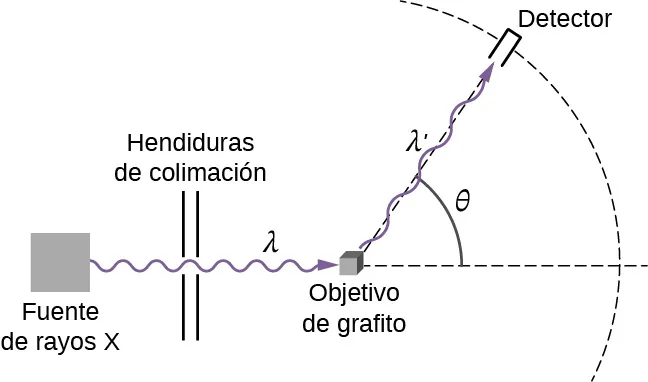
\includegraphics[width=.3\textwidth]{Images/Imagen_2.png}
      \end{center}
\end{wrapfigure}

El efecto Compton es el término utilizado para un resultado
inusual observado cuando los rayos X se dispersan en
algunos materiales. Según la teoría clásica, cuando una
onda electromagnética se dispersa de los átomos, se espera
que la longitud de onda de la radiación dispersada sea la
misma que la de la radiación incidente. En contra de esta
predicción de la física clásica, las observaciones muestran
que cuando los rayos X se dispersan en algunos materiales,
como el grafito, los rayos X dispersados tienen longitudes
de onda diferentes de las de los rayos X incidentes. Este
fenómeno clásicamente inexplicable fue estudiado
experimentalmente por Arthur H. Compton y sus
colaboradores, y Compton dio su explicación en 1923.

Para explicar el desplazamiento de las longitudes de onda
medido en el experimento, Compton utilizó la idea de
Einstein de la luz como partícula. El efecto Compton ocupa
un lugar muy importante en la historia de la física porque
demuestra que la radiación electromagnética no puede
explicarse como un fenómeno puramente ondulatorio. La
explicación del efecto Compton proporcionó un argumento
convincente a la comunidad física de que las ondas
electromagnéticas pueden comportarse en efecto como una
corriente de fotones, lo que situó el concepto de fotón en
una base sólida.

\begin{figure}[H]
      \begin{center}
            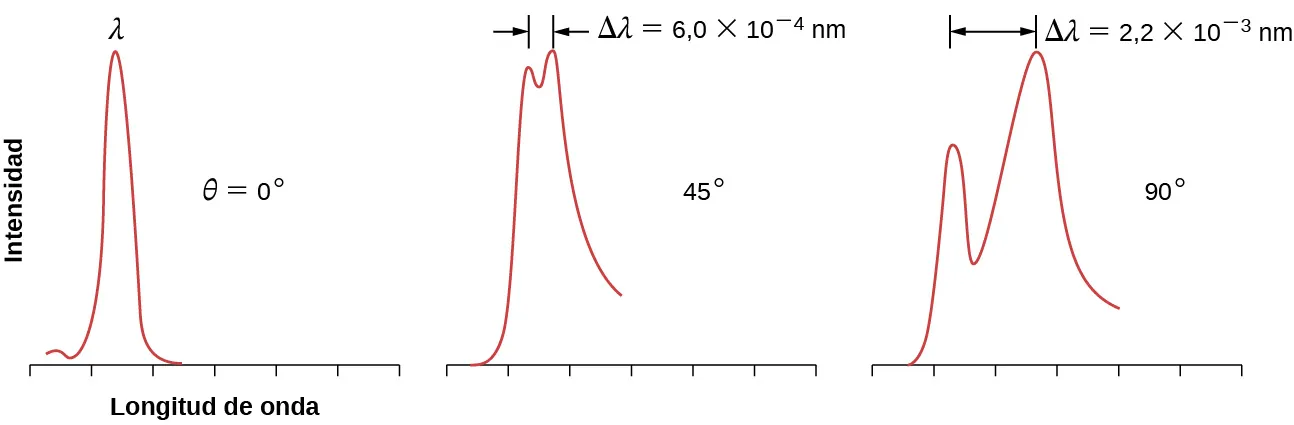
\includegraphics[width=.7\linewidth]{Images/Imagen_3.png}
            \caption{}
      \end{center}
\end{figure}

% + -------------------------------------------------------------|>
\subsection{Perdida de energía de un fotón~\cite{Tomé_2019}}

\begin{wrapfigure}{l}{.4\textwidth}
      \begin{center}
            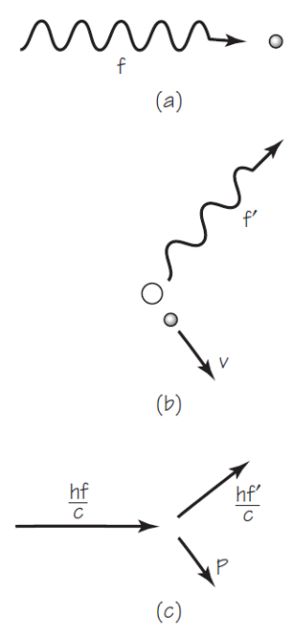
\includegraphics[width=.3\textwidth]{Images/Imagen_4.png}
      \end{center}
\end{wrapfigure}

Arthur Compton calculó cuánta energía debería perder un
fotón en una colisión con un átomo si el momento del fotón
fuese $\frac{h}{\lambda}$. Llegó a la conclusión de que el
cambio en la energía es demasiado pequeño como para poder
observar el efecto mecánico de un fotón en algo tan grande
comparativamente como un átomo completo. Pero si un fotón
golpeara un electrón, que tiene una masa significativamente
más pequeña, el fotón debería transferir una cantidad
significativa de energía al electrón.

En 1923, Compton pudo demostrar que los rayos X se
comportan de hecho como corpúsculos con momento lineal $p =
      \frac{h}{\lambda}$ cuando chocan con electrones. Compton
midió la longitud de onda (o la frecuencia) de los rayos X
incidentes y una vez dispersados y, de esta manera, pudo
determinar el cambio en el momento lineal del fotón de
rayos X. Al medir por separado el momento lineal del
electrón tras la dispersión, pudo verificar que $p =
      \frac{h}{\lambda}$ utilizando la ley de conservación del
momento.

% ! ----------------------------------------------------------------------|>
\section{Montaje Experimental}

\begin{itemize}
      \item Sensor-CASSY
      \item CASSY Lab 2
      \item Unidad MCA
      \item Preparado mixto $\alpha$, $\beta$, $\gamma$
      \item Equipo para efecto Compton
      \item Preparado de Cs-137, 3,7 MBq
      \item Contador de centelleo
      \item Etapa de salida de detector
      \item Fuente de alimentación de alta tensión 1,5 kV
      \item PC con Windows XP/Vista/7
\end{itemize}

\begin{figure}[H]
      \begin{center}
            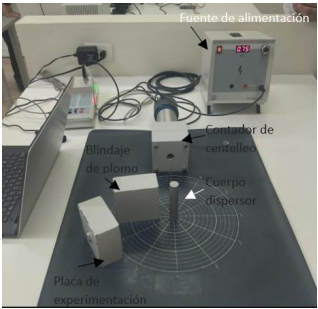
\includegraphics[width=.6\linewidth]{./Images/Fig.Montaje_1.png}
            \caption{}
      \end{center}
\end{figure}

% ! ----------------------------------------------------------------------|>
\section{Datos Experimentales}

\begin{table}[H]
      \begin{center}
            \begin{tabularx}{.5\linewidth}{|>{\centering\arraybackslash}X|>{\centering\arraybackslash}X|}
                  \hline
                  Grados & Energía Dispersada \bolditalic{(keV)} \\\hline
                  $0$    & $656.38$                              \\\hline
                  $30$   & $541.21$                              \\\hline
                  $60$   & $382.97$                              \\\hline
                  $90$   & $286.16$                              \\\hline
                  $120$  & $214.92$                              \\\hline

            \end{tabularx}
      \end{center}
\end{table}

% ! ----------------------------------------------------------------------|>
\section{Análisis de datos}

% + -------------------------------------------------------------|>
\subsection{}

\begin{figure}[H]
      \begin{center}
            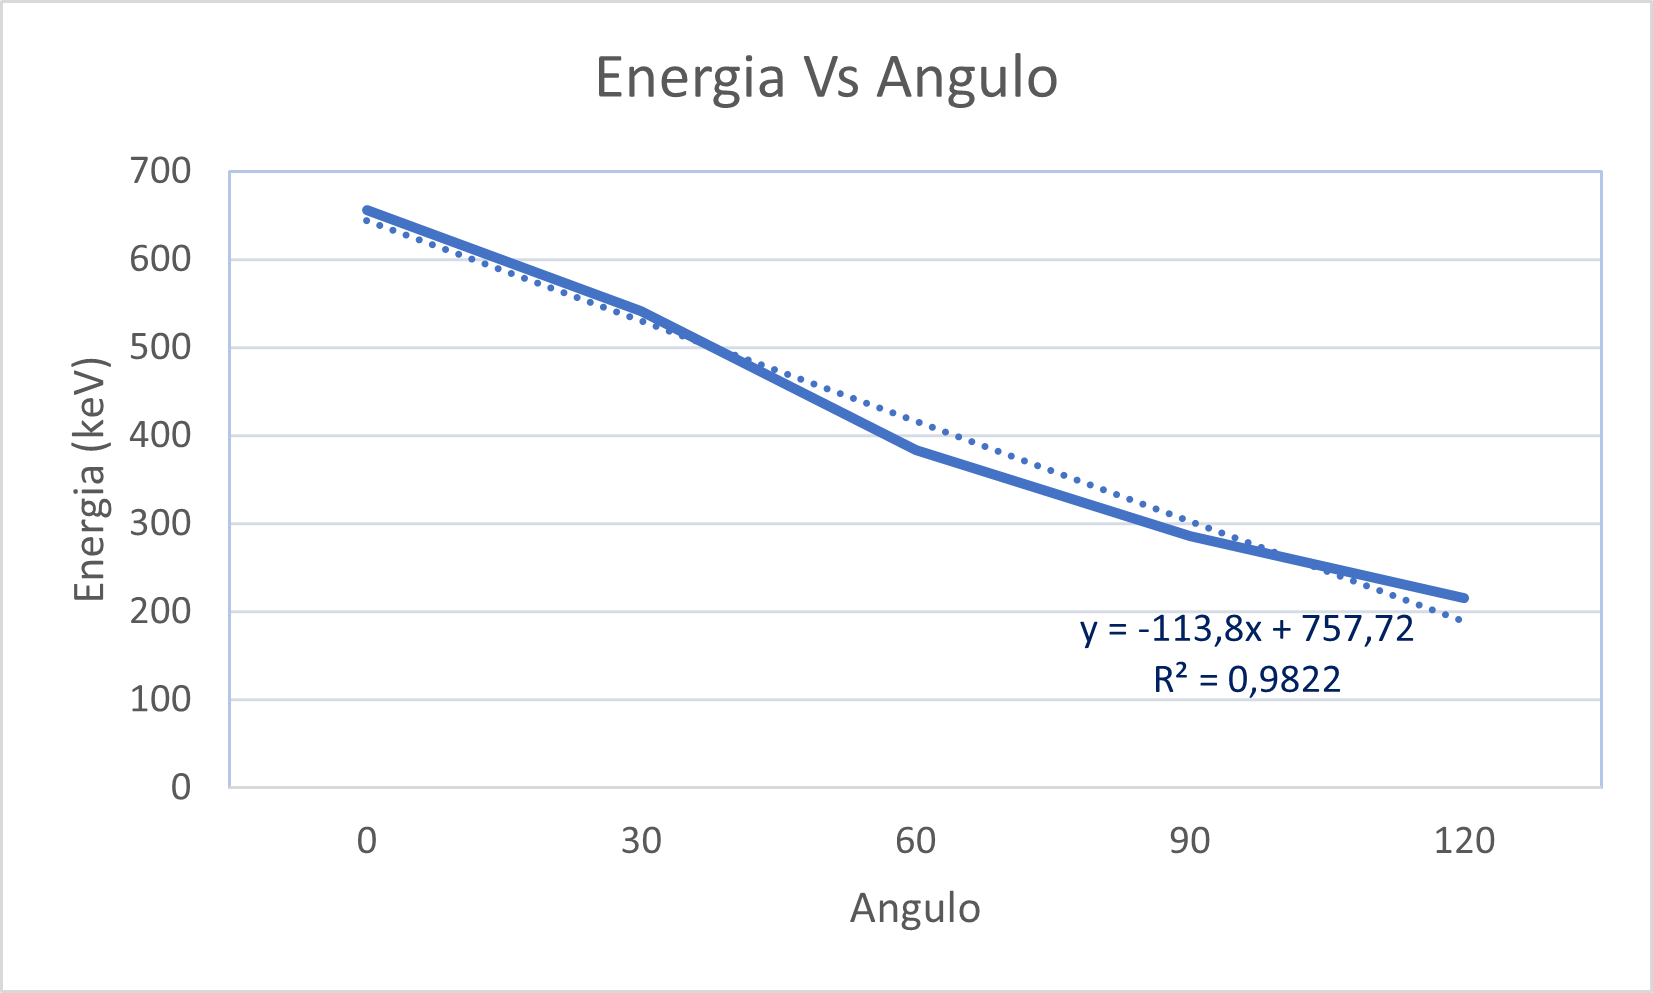
\includegraphics[width=.8\linewidth]{./Images/Graph.Analisis_1.png}
            \caption{}
      \end{center}
\end{figure}

Energía Promedio: $416.328$

Utilizando la formula,

\begin{equation*}
      \begin{gathered}
            E = \frac{h c}{\lambda} \\
            \lambda = \frac{h c}{E} \\
            \lambda = 2.9796 \times 10^{-12} m
      \end{gathered}
\end{equation*}

% + -------------------------------------------------------------|>
\subsection{}

Utilizando la formula,

\begin{equation}
      E_{2} = \frac{E_{1}}{1 + \frac{E_{1}}{m_0 \cdot c^{2}} \cdot (1 - \cos(\theta))}
      \label{eq:E2}
\end{equation}

\begin{table}[H]
      \begin{center}
            \begin{tabularx}{.8\linewidth}{|>{\centering\arraybackslash}X|>{\centering\arraybackslash}X|}
                  \hline
                  Angulo & Energía de los fotones dispersados \bolditalic{(eV)} \\\hline
                  $0$    & $6.56 \times 10^{5}$                                 \\\hline
                  $30$   & $6.11 \times 10^{-13}$                               \\\hline
                  $60$   & $1.64 \times 10^{-13}$                               \\\hline
                  $90$   & $8.19 \times 10^{-14}$                               \\\hline
                  $120$  & $5.46 \times 10^{-14}$                               \\\hline

            \end{tabularx}
      \end{center}
\end{table}

% + -------------------------------------------------------------|>
\subsection{}

Con base en los datos de energía de los fotones
dispersados, se puede concluir que la ecuación para el
efecto Compton se cumple. Esto se sustenta en el hecho de
que los valores calculados mediante la
ecuación~(\ref{eq:E2}) están dentro del rango teórico
esperado de la misma.

% + -------------------------------------------------------------|>
\subsection{}

\begin{table}[H]
      \begin{center}
            \begin{tabularx}{.8\linewidth}{|>{\centering\arraybackslash}X|>{\centering\arraybackslash}X|}
                  \hline
                  Grados & $\Delta \lambda$ \bolditalic{(m)} \\\hline
                  0      & $0          $                     \\\hline
                  30     & $3.25367 \times 10^{-13}$         \\\hline
                  60     & $1.21429 \times 10^{-12}$         \\\hline
                  90     & $2.42857 \times 10^{-12}$         \\\hline
                  120    & $3.64286 \times 10^{-12}$         \\\hline

            \end{tabularx}
      \end{center}
\end{table}

% + -------------------------------------------------------------|>
\subsection{}

\begin{figure}[H]
      \begin{center}
            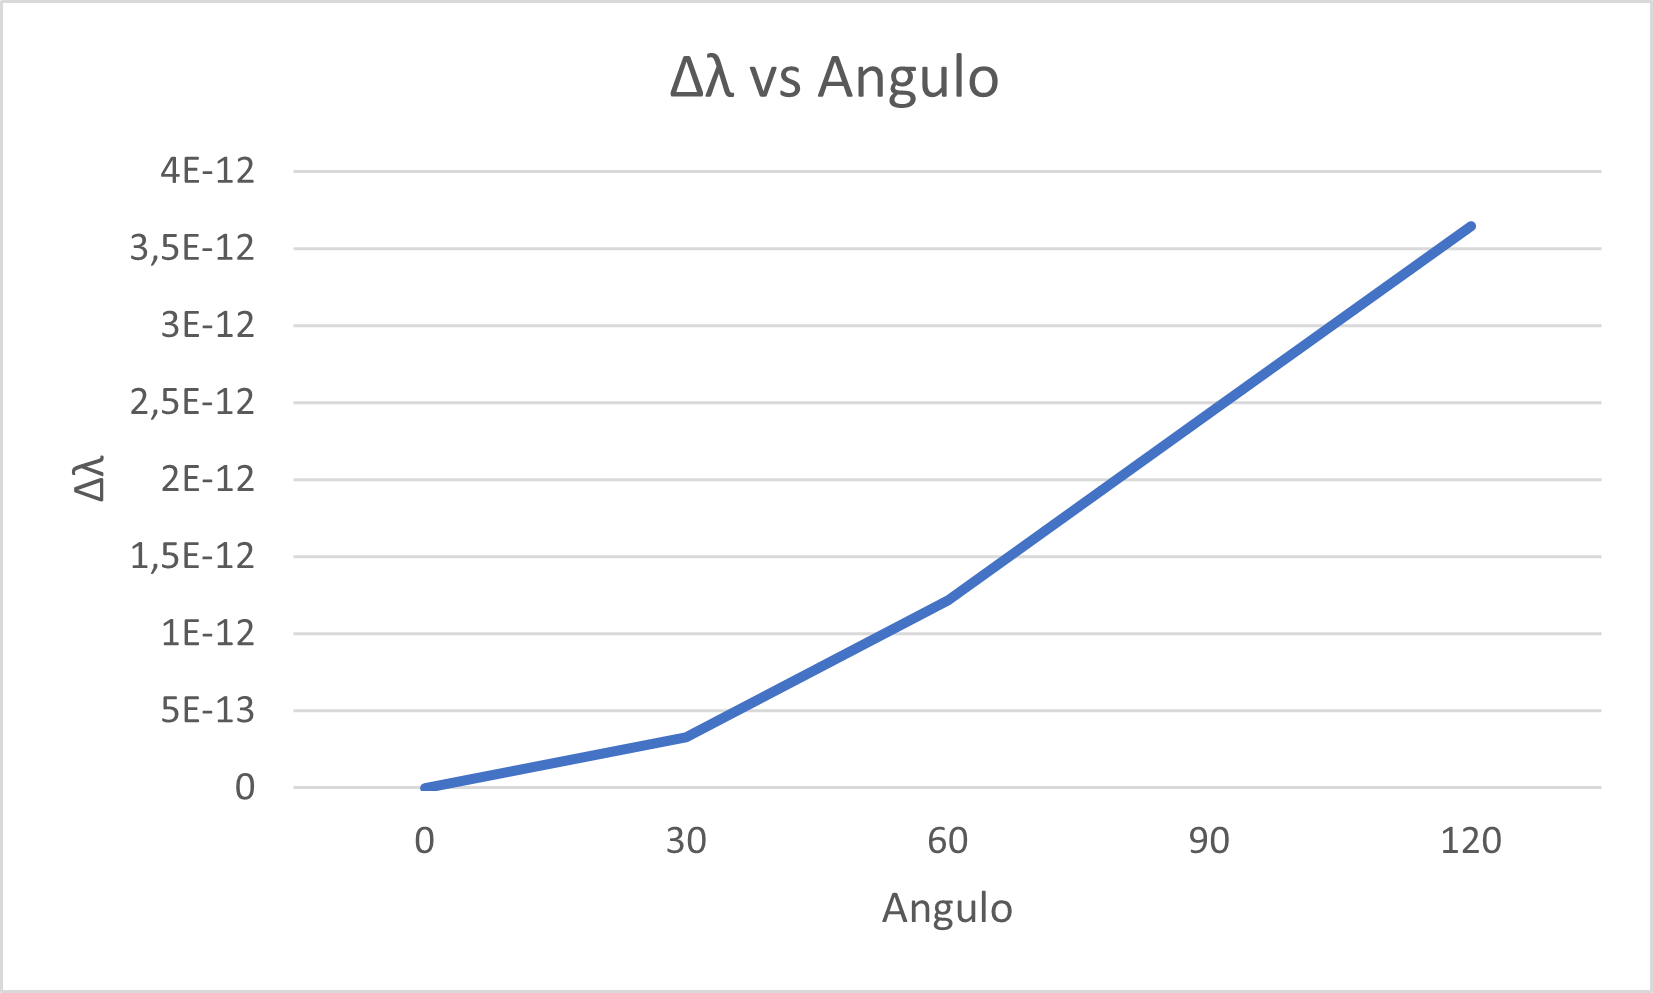
\includegraphics[width=.8\linewidth]{./Images/Graph.Analisis_2.png}
            \caption{}
      \end{center}
\end{figure}

% + -------------------------------------------------------------|>
\subsection{}

La función que mas se ajusta a la gráfica es,

\begin{equation*}
      y = 9 \times 10^{-13} x - 1 \times 10^{-12}
\end{equation*}

% + -------------------------------------------------------------|>
\subsection{}

\begin{figure}[H]
      \begin{center}
            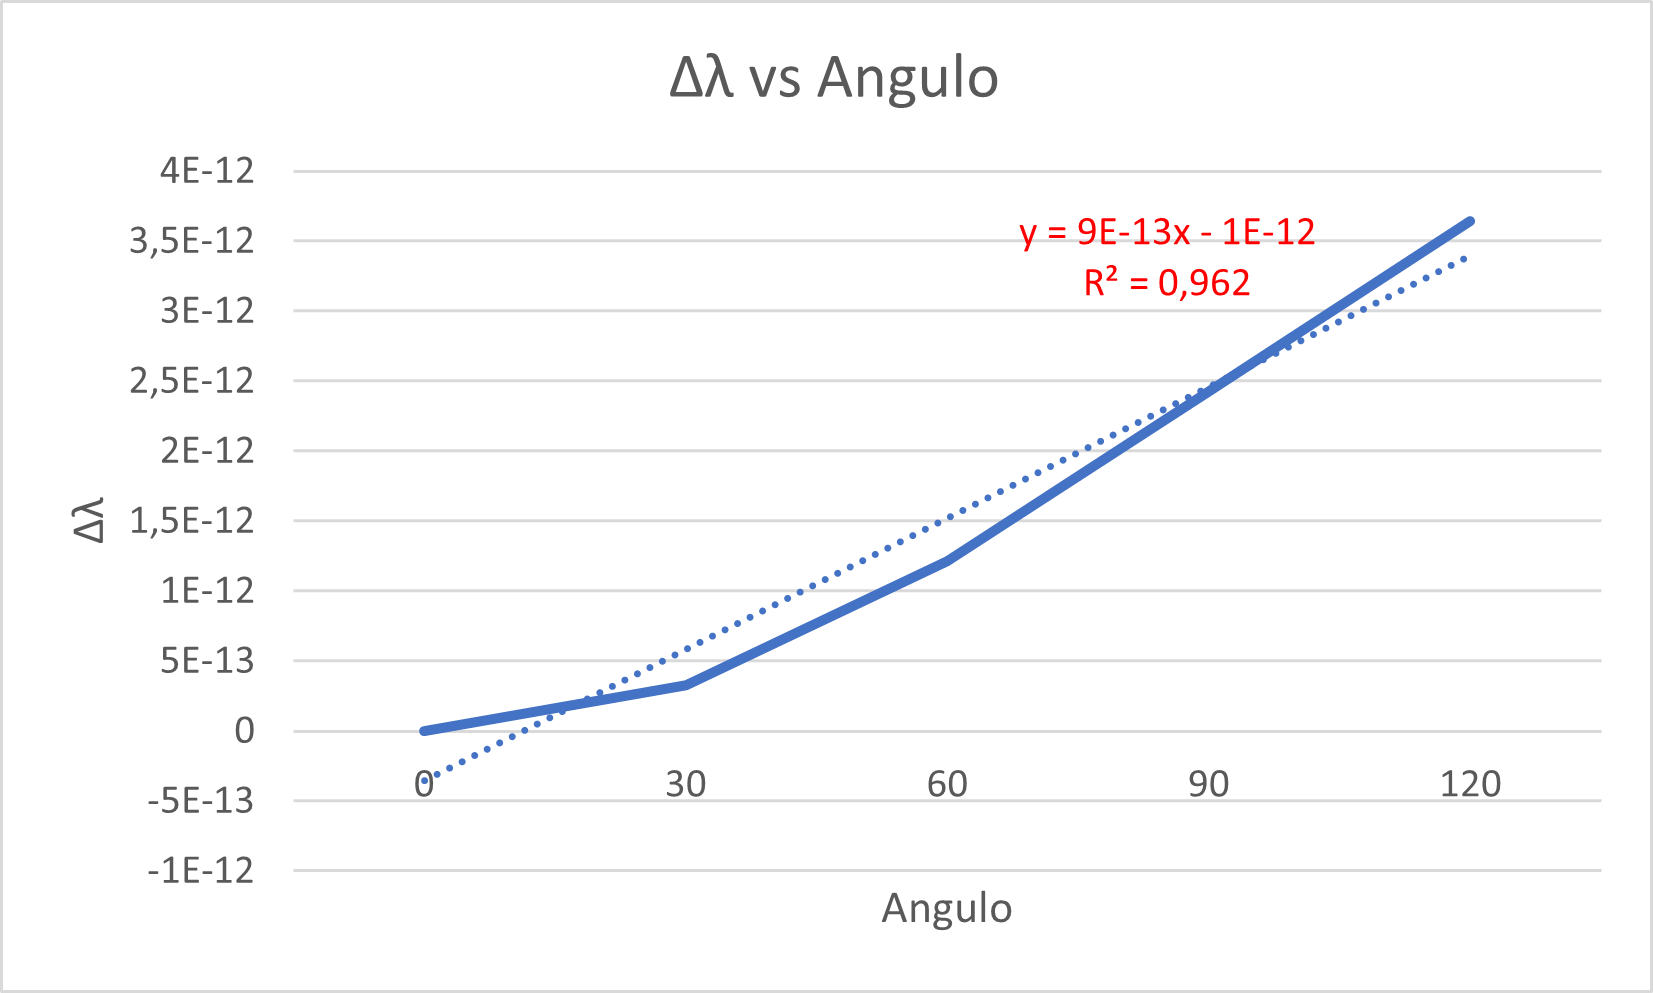
\includegraphics[width=.8\linewidth]{./Images/Graph.Analisis_3.png}
            \caption{}
      \end{center}
\end{figure}

% + -------------------------------------------------------------|>
\subsection{}

\begin{table}[H]
      \begin{center}
            \begin{tabularx}{.8\linewidth}{|>{\centering\arraybackslash}X|>{\centering\arraybackslash}X|}
                  \hline
                  Grados & \bolditalic{(\%)}     \\\hline
                  0      & 0                     \\\hline
                  30     & $9.87 \times 10^{01}$ \\\hline
                  60     & $9.77 \times 10^{01}$ \\\hline
                  90     & $9.70 \times 10^{01}$ \\\hline
                  120    & $9.66 \times 10^{01}$ \\\hline

            \end{tabularx}
      \end{center}
\end{table}

% ! ----------------------------------------------------------------------|>
\section{Conclusiones}

La practica experimental confirmo la validez del efecto
Compton, demostrando la variación en la energía y longitud
de onda de la radiación gamma dispersada. Los cálculos
experimentales respaldaron las expresiones teóricas,
proporcionando una verificación cuantitativa del fenómeno.
La relación entre el cambio en la longitud de onda y el
angulo de dispersion se ajusto a la formulación teórica,
permitiendo la determinación precisa de la Longitud de Onda
Compton para el electron. Estos resultados contribuyen a
fortalecer la comprensión de la naturaleza cuántica de la
radiación electromagnética.

\newpage

\printbibliography

\end{document}